\section{Data Binding. JCRContainer}
As it was discussed in the previous chapters - Magnolia CMS is closely connected
with Java Content Reporitory which is used as a storage. Development of a
convenient interface for JCR access is a crucial task As long as most of the
system data resides in JCR repository. In order to connect Vaadin components
widely used in the project with JCR we will design an implementation of Vaadin
Conatiner interface that operates on Java Content Repository workspaces and nodes.

\subsection{Vaadin Data Model}

Vaadin framework provides a versatile API allowing for binding user interface
components such as fields and tables to an underlying data storage. The possible
type of such a storage varies from POJO's and property files to the database
queries. In our case it will be represnted by a Java Content Repository query.

The base interfaces of the API reside in \texttt{com.vaadin.data} package.
Figure \ref{fig:vaadin_data_binding} describes the main layers involved into
connecting the data with a UI \cite{vaadin_data_model}:
\texttt{Property}, \texttt{Item} and \texttt{Container}.

\begin{figure}[H]
	\centering
	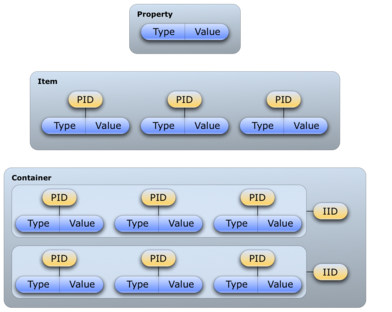
\includegraphics[width=\textwidth]{impl/vaadin_data_binding.png}
	\caption{Vaadin Data Model}
	\label{fig:vaadin_data_binding}
\end{figure}

\subsubsection{Property}
\texttt{Property} is a basic used in Vaadin data binding mechanism.
\texttt{Property} is used for binding a single data value of an
arbitrary type. The main purpose of it is to provide the univeral value management 
interface allowing to set and retreive it. Properties are also optionally
capable of notifying about the underlying value change\cite{vaadin_data_model}.

Properties are not responsible of mapping themselves to any identifiers in case
of complex data-set bindings. It a job of an \texttt{Item} to associate a
\emph{Property Identifier} or \emph{PID}. Using the tabular structure analogy a
\texttt{Property} value corresponds to a single cell whereas its PID would act
as a column name \cite{vaadin_data_model}.

\subsubsection{Item}
As it was discussed before an \texttt{Item} concept is used to organize a set of
properties associated with some sort of an identifier. In the object-oriented
programming paradigm items would correspond to objects providing simple yet
rather powerful introspection meachism:
properties can be obtained by an identifier (\texttt{getItemProperty(id)}
method), additional properties can be appended or removed during the run-time
(\texttt{addItemProperty()} and \texttt{removeItemProperty()} methods). Items
normally notify the subscribers of type \texttt{PropertySetChangeNotifier} with
\texttt{PropertySetChangeEvent} of the changes of an internal structure. In
tabular data-structures an item corresponds to a single row entry.

\subsubsection{Container}
The top-most interface of Vaadin data-binding model is \texttt{Container}.
Containers manage the sets of \texttt{Items} which usually have a similar
structure (same or close to similar set of \texttt{Properties}). Whereas the
primary goal of a \texttt{Container} is to manage a set of items associating
them to identifiers, containers can also provide advanced approaches of data
manipulation, e.g. hierarchical relations, ordering, sorting and filtering.
Containers are used in Vaadin framework as the data providers for such
components as trees, tables and selection fiedls \cite{vaadin_data_model}.

\subsection{Mapping JCR API to Vaadin Data Model}
In order to design an efficient Vaadin container that operates over Java Content
Repository we first have to define a clear relation between the basic
abstractions of the two interfaces.

According to the specification of the JCR \cite{jcr_specification} the
repository has a tree-like structure with the \texttt{javax.jcr.Node} objects as
elements of the tree and \texttt{javax.jcr.Property} objects as the tree leaves.
Both of these interfaces are the children of \texttt{javax.jcr.Item} interface.
\texttt{javax.jcr.Node} may contain either the sub-nodes and the properties.  
Each node is assigned with a \emph{node identifier} (\emph{uuid}), whereas the property
uses its name as an identifier.

Thus, we can conclude that there is a natural mapping between the repository
structure and \texttt{com.vaadin.data.Container}: both manage a set of items
operating over them by means of an associated identifier mechanism. Advanced
Vaadin container operations such as sorting, filtering and ordering can be
fulfilled with JCR Query API.

In addition to that we can map the \texttt{javax.jcr.Node} interface to
\texttt{com.vaadin.data.Item} as they play rather simlar roles - handling a set
of underlying properties. The case of \texttt{javax.jcr.Property} has to be
examined more carefully: on the one hand it is capable of managing a single
value and functionally resemble the \texttt{com.vaadin.data.Property}, on the
other hand - they are treated equally to the nodes in repostory structure. This
complication leads us to the decision to map \texttt{javax.jcr.Property} to the
Vaddin Item interface as well as the nodes. However, it has to be reflected in
the implementation that this kind of an \texttt{com.vaadin.data.Item} is a
special case and it is capable of managing one and only one property. 

\subsection{JcrContainer}
Let us examine the structure of the \texttt{JcrContainer} that binds Vaadin Data Model to the 
Java Content Repository.

\begin{figure}[H]
	\centering
	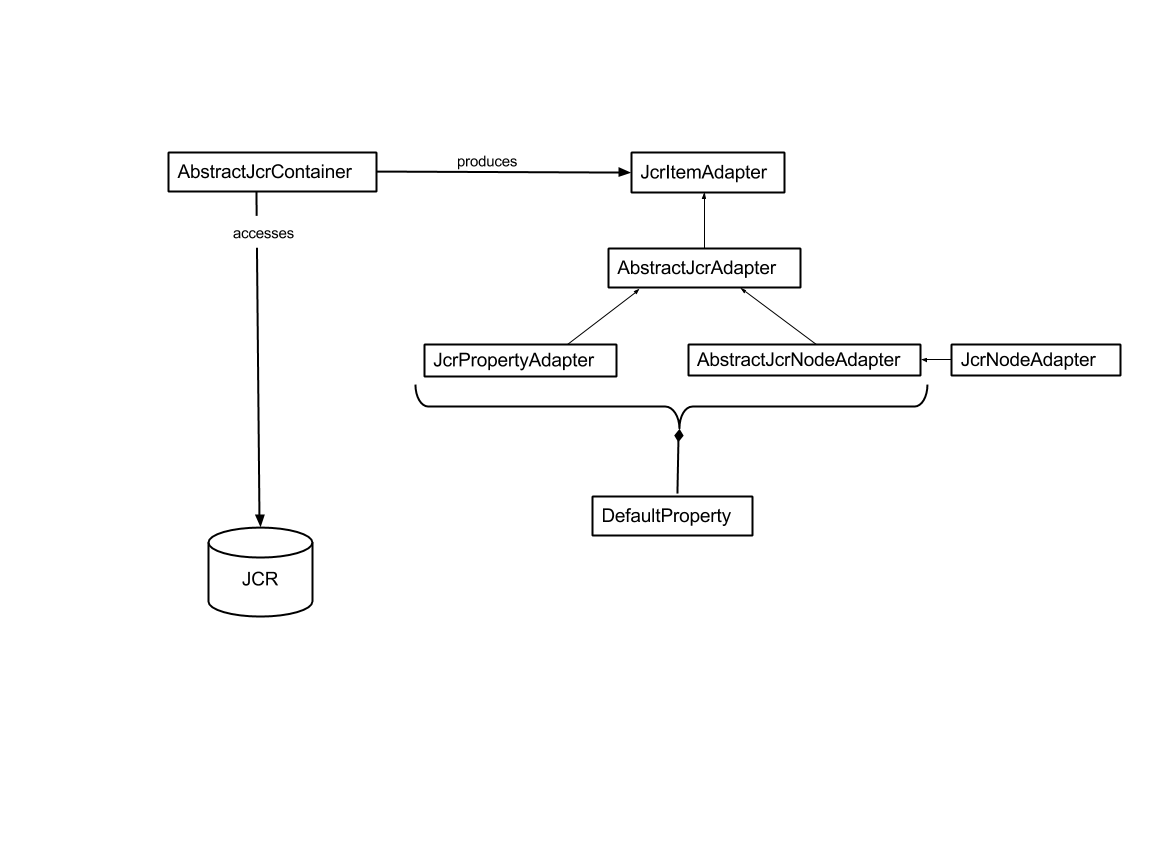
\includegraphics[width=\textwidth]{impl/jcr_container.png}
	\caption{JcrContainer}
	\label{fig:jcr_container}
\end{figure}

\begin{itemize}
  \item \texttt{DefaultProperty} is a simple in-memory Vaadin property
  implementation that does not directly accesses JCR.
  \item \texttt{JcrItemAdapter} provides a common interface for JCR nodes and
  properties to be accessed as Vaadin items. The implementors of this interface
  wrap and manage the correspondent jcr items. \texttt{DefaultProperty} is used to buffer
  the data retreived from a repository and to postpone the write operations as
  long as possible.
  \item \texttt{AbstractJcrCotainer} implements Vaadin \texttt{Container}
  interface and accesses JCR in order to retreive JCR items and construct the
  correspondent wrappers. As the volume of the data stored in JCR repository is
  not bound above we have to ensure that our container is scalable in the
  sense that it does not load the items unless their contents are explicitly
  queried and that it does not store more items than a certain threshold. Thus,
  \texttt{AbstractJcrCotainer} maintains an internal limited cache of items
  loaded in memory.
\end{itemize}
 

